\subsection{Synchrotron x--ray source and ray tracing}
The synchrotron x--ray source and propagation from the source to the target is
realized with the
\href{http://ftp.esrf.eu/pub/scisoft/Oasys/readme.html}{\textit{Oasys}}
software package using the x--ray tracing
code \textit{Shadow3}. Installation scripts and the wiki page for \textit{Oasys} can be
found at
\href{https://github.com/srio/oasys-installation-scripts/wiki}{https://github.com/srio/oasys-installation-scripts/wiki}.
\href{https://github.com/srio/ShadowOui-Tutorial}{Tutorials for
Oasys and ShadowOUI} cover the various steps in preparing, executing, and
analysing the raytracing simulation. As part of preparation for the new High Power
Laser Facility (HPLF), that will be installed on the ID24 beamline at the ESRF,
the current energy dispersive x--ray absorption beamline has been simulated using
\textit{Oasys}.
The ID24 beamline workflow for \textit{Oasys} can be obtained from the EUCALL Data
Repository at Zenodo \cite{Briggs2017.zenodo.886451}.

\subsection{Particle matter interaction: long pulse laser}
The long pulse laser interaction with sample is performed using the \textit{Esther} hydrocode.
Here we have demonstrated an experiment that could be performed on the
ID24 \gls{xas} beamline, where a \SI{6}{\nano\second} flat top laser pulse (wavelength
\SI{1064}{\nano\metre}) sends an ablative
driven shockwave through a \SI{45}{\micro\metre} CH-plastic ablator and into a
\SI{5}{\micro\metre|} Fe layer. A
tutorial that describes how the input files are generated (and how output data is
obtained) is provided on the
\href{https://www.github.com/eucall-software/simex_platform/wiki/Esther-Hydrocode-Tutorial}{Simex
wiki page}; all example input
and output files are available from the Ref.~\cite{Briggs2017.zenodo.883106}.
The pressure in the Fe sample at $t = \SI{8.9}{\nano\second}$
(laser pulse begins at $t = \SI{0}{ns}$) is shown in Fig.~\ref{fig:hydro}.

 The pressure, temperature, density and velocity can all be obtained at a given
 time step from the output files that Simex converts to opmd format. Upon
 completion of the code, it is then possible to adjust laser parameters to reach
 different pressure-temperature conditions in the Fe sample. The P-T condition
 where the pressure is uniform through the whole of the sample is then stored and
 \gls{xas} modelling can be performed to simulate the expected E\gls{xafs} signal at
 the compressed state.
%
 \begin{figure}
   \centering{%
     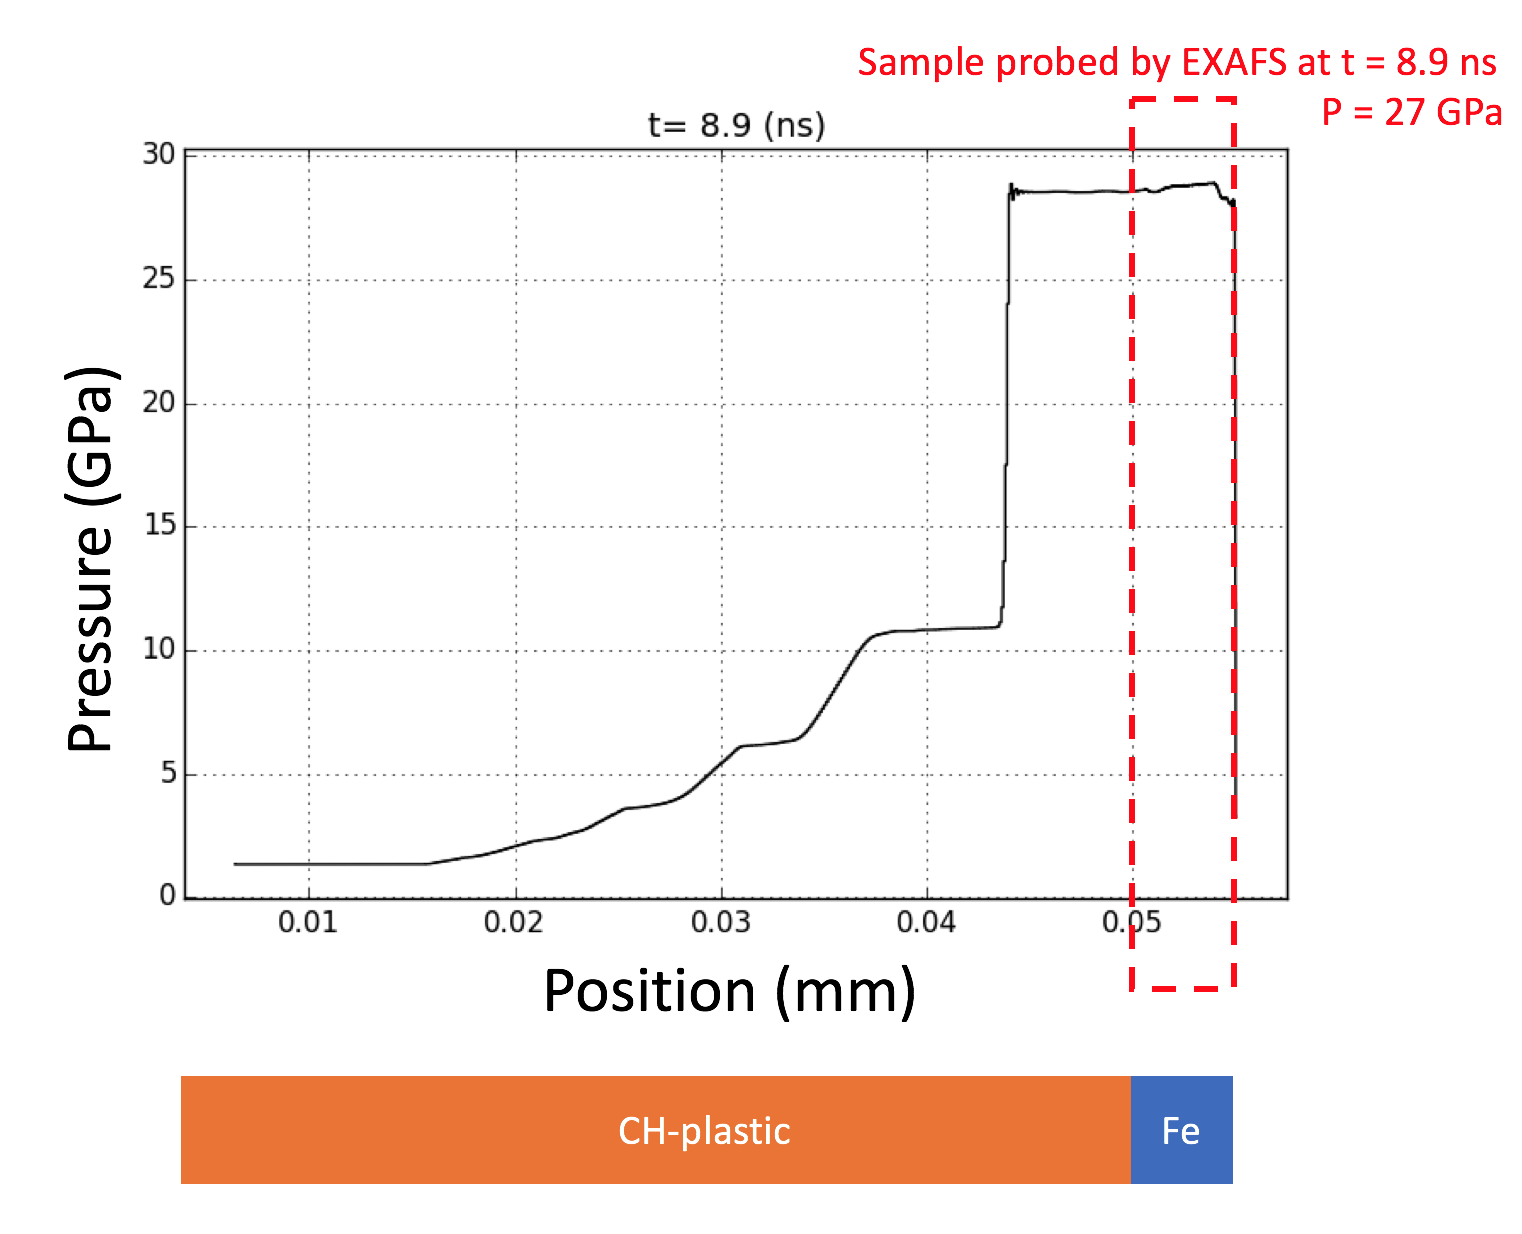
\includegraphics[width=4.822in]{figures/SIMEX-Fe-Shock.png}
     \caption{%
       Pressure wave in the iron target and plastic ablator layer. The red--dashed
       box is the range probed by \gls{exafs}.  \label{fig:hydro}}
   }
 \end{figure}
%
 \subsection{Modelling of \gls{exafs}}
In this simple example, to show the interoperability with the hydrocode,
we run through the requirements that are necessary for
simulation (fitting) of \gls{exafs} data relevant to a sample experiment obtain signal
from a \SI{5}{\micro\metre} thick Fe foil. The simulation will be carried out for
ambient conditions Fe foil; a future enhancement of SIMEX will take P-T
conditions from hydrocode simulations before performing high-pressure
\gls{xanes}/\gls{exafs} calculations.

To validate the \gls{exafs} simulations, we compare the simulated spectrum with raw
data obtained from an \gls{xas} beamline at the ESRF synchrotron. The
normalized \gls{xas} spectrum for a \SI{5}{\micro\metre} thick Fe foil is shown in
Fig.~\ref{fig:hydro}.
%
\begin{figure}
  \centering{%
    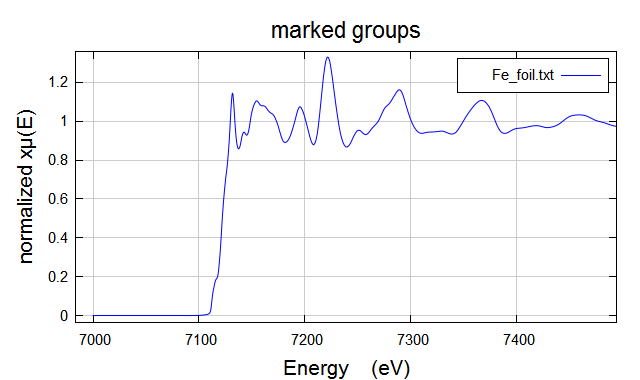
\includegraphics[width=4.822in,height=2.528in]{figures/Task42210-img001.png}
    \caption{%
      X--ray absorption spectra collected at BM23 (\gls{exafs} beamline, ESRF) of
      a \SI{5}{\micro\metre} thick iron foil.
      \label{fig:xafs_spectra}
    }
  }
\end{figure}
%
Calculations of \gls{xafs} spectra are performed using the \textit{FEFF} package. \textit{FEFF} uses a
single input file to select which modules should be run inside the program and
what parameters should be used. The material of interest is contained within
this input file based on its crystallographic parameters and atomic positions.
The \textit{ATHENA} program is able to combine crystallographic input files (.cif format)
for a chosen material into the \textit{FEFF} .inp format. The .cif files can be
found on crystallographic database websites or can be manually created
using gui programs such as \textit{VESTA}. \textit{FEFF} is then run to
calculate the scattering paths
between atoms and the run data is then exported for use by other third party programs
(such as \textit{ARTEMIS}) to compare with experimental data.
A comprehensive user guide for running ARTEMIS
/ \textit{FEFF} can be found at\\
\href{http://bruceravel.github.io/demeter/artug/index.html}{http://bruceravel.github.io/demeter/artug/index.html}.
%
\begin{figure}
  \centering{%
    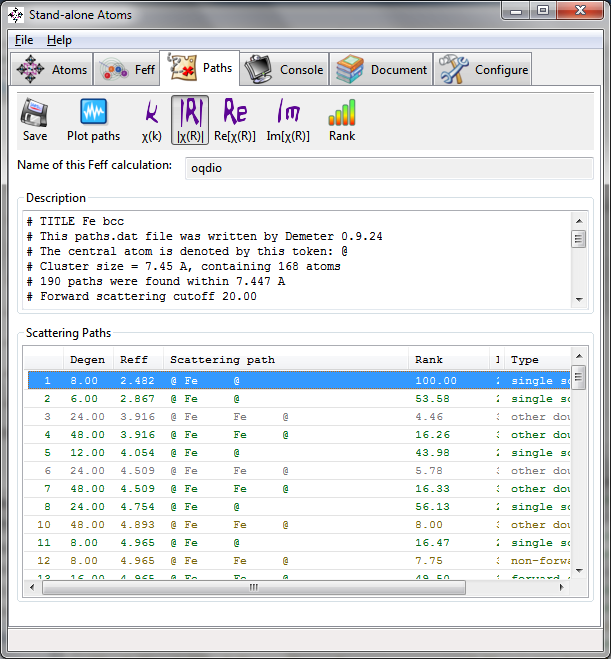
\includegraphics[width=4.3063in,height=4.6465in]{figures/Task42210-img002.png}
    \caption{%
      Screenshot of the output data collected in the ATOMS software after
      running \textit{FEFF} simulation of iron at ambient conditions.
      \label{fig:xafs_fig2}
    }
  }
\end{figure}
%
\begin{figure}
  \centering{%
    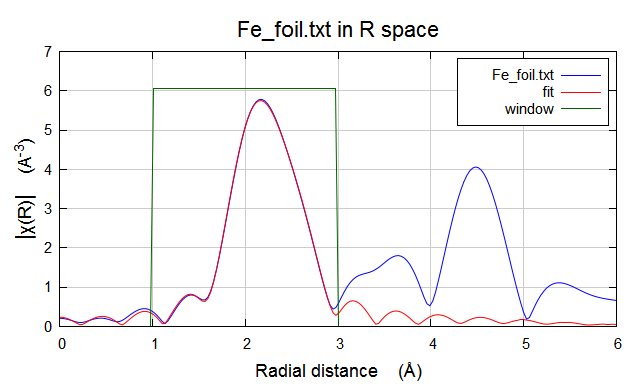
\includegraphics[width=4.852in,height=2.9173in]{figures/Task42210-img003.png}
    \caption{%
      Fitting of the first Fe shell from \textit{FEFF} calculations (red) to Fe
      \gls{exafs}
      data collected on BM23 beamline, ESRF (blue).
      \label{fig:xafs_fig3}
    }
  }
\end{figure}
%
\subsubsection{Simulating \gls{xanes} at shock conditions}
Shock compression experiments on Fe have previously been carried out at the ESRF
\cite{Torchio2016}. In that study,
simulations of the \gls{xanes} at shock conditions were carried out using the
\textit{abinit} code and are shown below in Fig.~\ref{fig:xafs_fig4}.
%
\begin{figure}
  \centering{%
    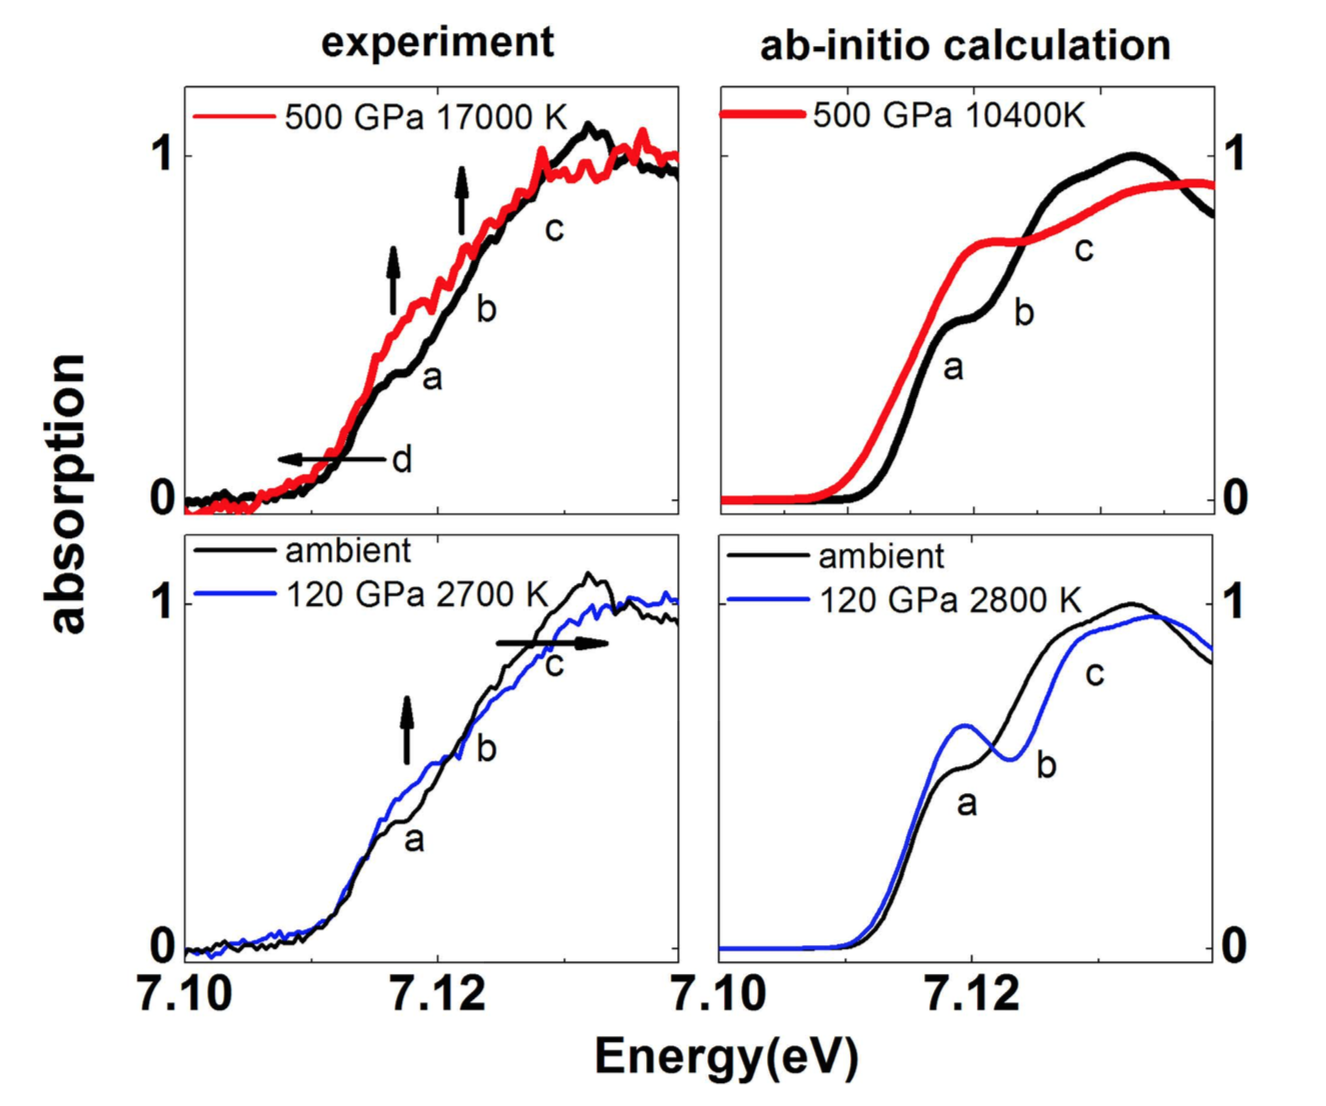
\includegraphics[width=4.3063in,height=3.5945in]{figures/Task42210-img004.png}
    \caption{%
      Comparisons of the absorption edge of Fe between experiments (left
      panels) and ab-initio calculations (right panels) at
      \SIlist{120;150}{\giga\pascal}. Figure
      taken from Ref.~\cite{Torchio2016}.
      \label{fig:xafs_fig4}
    }
  }
\end{figure}
